\exam{Exercises 1}
\question{Problem 1}
\begin{equation*}
	f(x)=\sin(10x)+\cos(3x)
\end{equation*}
\questionitem{Item a}
Within the interval $[3,6]$ there are 9 roots.
\begin{center} 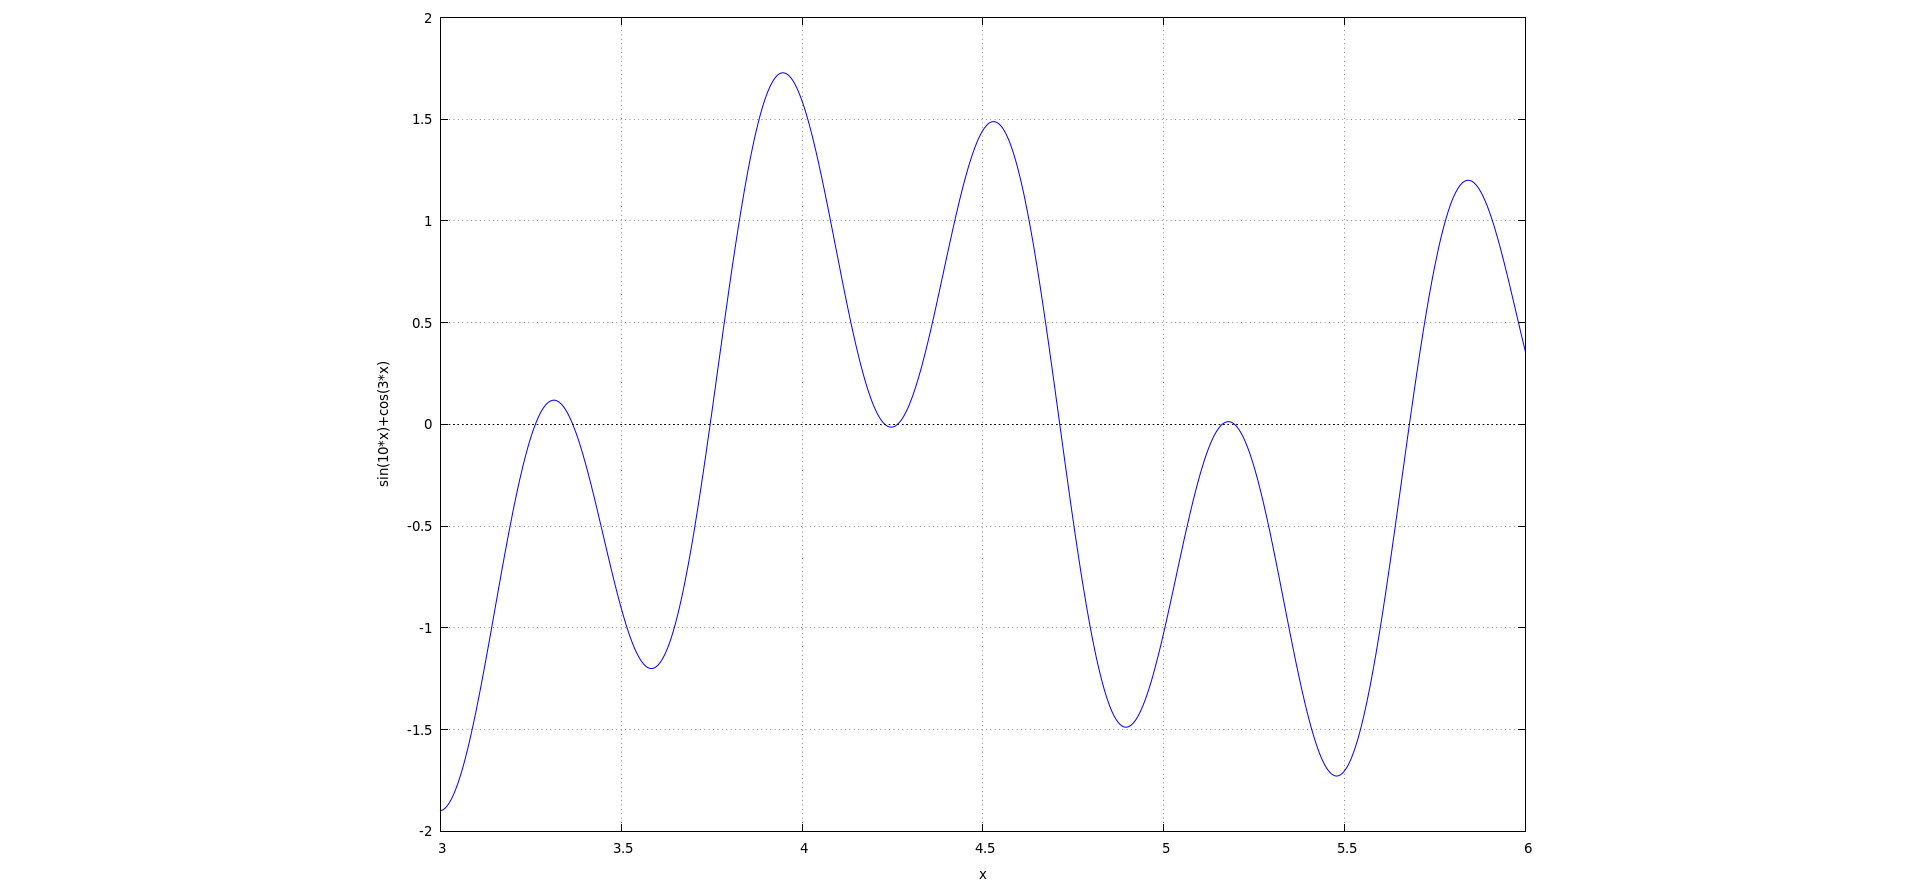
\includegraphics[height=60mm,keepaspectratio]{EXER1T1-1-a} \end{center}

\questionitem{Item b}
The lowest root is in the interval $[3.2,3.3]$ and the highest root is in the interval $[5.6,5.7]$.
\newpage

\questionitem{Item c}
\begin{center}
\begin{tabular}{ p{73mm} p{0mm} p{73mm} }
	Bisection & & False position \\
	\lstinputlisting[language=C++, caption=EXER1T1-1c\_bisection (C++)]{EXER1T1-1-c_bisection.cpp} & &
	\lstinputlisting[language=C++, caption=EXER1T1-1c\_falsepos (C++)]{EXER1T1-1-c_falsepos.cpp}
\end{tabular}
\end{center}
\lstinputlisting[caption=Input EXER1T1-1c]{EXER1T1-1-c.in}
\begin{center}
\begin{tabular}{ p{73mm} p{0mm} p{73mm} }
	\lstinputlisting[caption=Output EXER1T1-1c\_bisection,basicstyle=\small]{EXER1T1-1-c_bisection.res}
	& &
	\lstinputlisting[caption=Output EXER1T1-1c\_falsepos,basicstyle=\small]{EXER1T1-1-c_falsepos.res}
\end{tabular}
\end{center}
